\chapter{Súčasný stav}

Android je operačný systém ktorý je založený na licencii open source\cite{android}. To znamená, že hocikto môže bezplatne sťahovať a distribuovať jeho zdrojový kód. To dospelo do súčasného stavu, kedy má prístup k výkonným mobilným zariadeniam väčšia časť populácie ako kedykoľvek predtým. Každá spoločnosť si môže upraviť Android podľa vlastných predstáv a poskytnúť zákazníkovi jedinečné prostredie. Okrem toho získali vývojári prístup k veľkému publiku, keďže vývojári nemuseli platiť za licencie, alebo vyvíjať vlastný operačný systém. To umožnilo vývojárom znížiť náklady na vývoj a od roku 2011 do 2013 klesla priemerná cena smartphonov na celom svete o 25\% \cite{cena_smartphone}. Pokiaľ by sme chceli stráviť jednu minútu prezeraním každého jedného zariadenia s Androidom, trvalo by nám to dva a pol týždňa bez spánku. Momentálne existuje na svete 24000 zariadení od takmer 1300 značiek \cite{pocetTelefonov}. Vďaka Androidu vznikli rôzne verzie, medzi ktoré patrí CyanogenMod, MIUI, AOKP momentálne je najpoužívanejšia verzia Androidu je 5.0-5.1 Lollipop s 32,5\% podielom na trhu \cite{usage}, ostatné verzie a ich podiel na trhu môžeme vidieť na grafe (obr.\ref{obr1.1}.)

\begin{figure}[ht]
    \begin{center}
        \begin{minipage}{0.99\linewidth}
            \begin{center}
                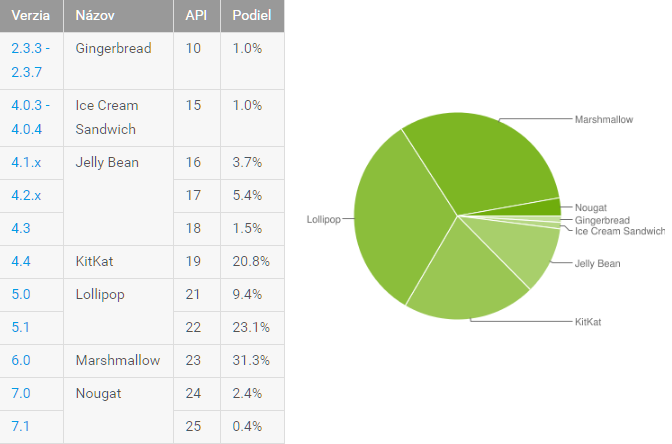
\includegraphics[width=0.99\textwidth]{images/verzie_and.png}
                \caption{Podiel verzií Androidu}
                \label{obr1.1}
            \end{center}
        \end{minipage}
    \end{center}
\end{figure}
 

Ponuka, ktorú nám Android prináša, nekončí pri počte zariadení, ale aj aplikáciami, ktorých je cez Google Play dostupných viac ako 1 milión \cite{android}. Dostupné sú aj alternatívy ku Google a to Amazon Appstore, GetJar, Mobogenie, SlideME, F-Droid \cite{playstore_alt}.

\section{História}

Spoločnosť Android Inc. bola založená v Palo Alto, California v Októbri 2003 \cite{history_android}.Pri vzniku stáli Andy Rubin, Rich Miner, Nick Sears a Chris Whie s myšlienkou vytvoriť múdrejšie mobilné zariadenia, ktoré by si boli vedomé o svojej pozícii a používateľových preferenciách. Pôvodný úmysel spoločnosti bol vyvinúť pokročilý operačný systém pre digitálne fotoaparáty,ale  malý trh ich naviedol na cestu vývoja pre mobilné zariadenia a konkurovať tak Symbianu a Windows Mobile. \cite{history_cameras}


\section{Verzie Androidu}
Najvyššie číslo dostupnej verzie operačného systému Android je \textit{7.0} a vzhľadom k tomu sa už staršie verzie vo veľkom počte nepoužívajú, preto sa budeme v nasledujúcich podkapitolách venovať len verziám s minimálnym podielom 15\%

\begin{description}
\item[KitKat] Vydaný v Októbri 2013 bol vylepšený oproti predošlým verziám  o nástroj na analýzu pamäte, nahrávanie obrazovky, API k infračervenému blastru a audio monitoring. Od tejto verzie majú vývojári prístup k SMS API. \cite{versions} . Dalšie podverzie 4.4.1 až 4.4.4 priniesli hlavne bezpečnostné opravy.


\item[Lollipop] Najväčšiu zmenu, ktorú Lollipop priniesol ku koncu roka 2014 do androidu  bol nový dizajn používateľského prostredia vybudovaný pomocou dizajnového jazyka \textit{Material Design} ktorý je hlavným vizuálnym prvkom Googlu. Virtuálny stroj Dalvik bol nahradený Android Runtime\cite{dalvik}. Lollipop 5.0.1 - 5.1.1, pridali podporu viacerých SIM a  ochranu zariadenia pri krádeži.


\item[Marshmallow] Pribudol správca povolení pre aplikácie. API ,ktoré umožňuje pristupovať k práve zobrazeným dátam na obrazovke. Od 6.0 Android natívne podporuje odtlačky prstov a USB-C a funkcia \textit{deep sleep}, ktorá pomáha šetriť batériu v prípade potreby.


\item[Nougat] Predstavil výrazné zmeny. Pribudla možnosť zobraziť viaceré aplikácie na jednej obrazovke, rozdelenie obrazovky na časti, instantné odpovede priamo v notifikačnom centre a optimalizačné prvky pre virtuálnu realitu.

\end{description}

\chapter{Použité technológie}

Operačný systém Android je naprogramovaný hlavne v jazyku Java \cite{android_code}  (tab. \ref{tab:android_code}), rovnako ako aj aplikácie. Pre vývoj je potrebné mať nainštalované JDK spolu s  SDK Manager, pomocou ktorého môžeme stiahnuť potrebné verzie Android SDK, obsahujúce nástroje , ktoré kompilujú kód spolu s inými časťami aplikácie ako sú obrázky, jazykové súbory do APK archívu , ktorý obsahuje všetky súbory potrebné na inštaláciu. Android je multi-user Linux systém, v ktorom je každá aplikácia definovaná ako používateľ. Každá aplikácia má priradené unikátne používateľské ID pomocou ktorého systém obmedzí povolenia pre aplikáciu.Každá aplikácia má svoj Linux proces, ktorý je vytvorený vždy. keď je potrebné spustiť komponent aplikácie, a je ukončený vždy keď proces nie je naďalej potrebný alebo systém potrebuje pamäť pre iné aplikácie.


\vspace{10pt}

\begin{table}[hb!]
    \centering
    \begin{tabular}{| l | l | }
    \hline
        Jazyk   &   Podiel kódu     \\  \hline
        Java    &   46,1\%          \\  \hline
        C       &   30,8\%          \\  \hline
        C++     &   13,4\%          \\  \hline
        Ostatné &   9,7\%           \\  \hline
    \end{tabular}
    \caption{Percentuálny podiel jazykov v AOSP}
    \label{tab:android_code}
\end{table}

\section{Nástroje}

Vývoj softvéru sa nezaobíde bez výberu správnych nástrojov. Nie sme nútení písať aplikácie v obyčajných textových editoroch, máme k dispozícií veľké množstvo prepracovaných vývojových nástrojov ktoré umožňujú rýchly re-faktoring kódu, analýzu kódu, build systémy pre ľahší a rýchlejší vývoj. Za nástroje považujeme aj súčasné technológie, ktoré uľahčujú prácu s rôznymi časťami aplikácie a poskytujú nám abstrakciu, ktorá umožní písať kvalitný a čitateľný kód.

\section{Android Studio}

Od 26.Júna.2015 prestal Google oficiálne vyvíjať plugin pre IDE Eclipse \cite{androidstudio} a Android Studio sa stalo jediným oficiálne podporovaným nástrojom na vývoj pre platformu Android. Na jeho vývoji sa podieľa Google a taktiež spoločnosť JetBrains ktorá vyvíja IntelliJ Idea, na ktorom je Android Studio založené. Medzi jeho výhody patria \cite{androidstudio2} 


\begin{itemize}

\item Build nástroj Gradle, ktorý automaticky zostavuje aplikáciu spolu s knižnicami, alebo inými projektami
\item Refaktoring špecifický pre Android
\item ProGuard ktorý zmenšuje veľkosť aplikácie, maže zbytočný kód a komplikuje reverzné inžinierstvo
\item Android špecifické šablóny
\item GUI editor 
\item Hĺbková analýza kódu

\end{itemize}

\section{IntelliJ Idea}

Android Studio a Android plugin pre IntelliJ Idea sú postavené na rovnakom kóde \cite{androidstudio3} pričom nedostaneme pred-konfigurovaný nástroj na vývoj priamo od inštalácie. Jedná sa o produkt, ktorý je primárne IDE pre Javu a J2EE. Projekty, vytvorené v Android Studio, je možné otvoriť v IntelliJ Idea a vice versa. Spoločnosť JetBrains poskytuje pluginy ktoré poskytujú lepšiu prácu s verzionovacím systémom alebo databázou.


\section{Kotlin}

Kotlin je staticky typovaný jazyk bežiaci nad JVM vyvíjaný \textit{JetBrains}, ktorý síce nie je syntakticky kompatibilný s Javou, ale je navrhnutý tak, že umožňuje využívať všetky Java knižnice. Narozdiel od  Javy si nevyžaduje veľa písania, podporuje lambda výrazy, dátové triedy a automaticky generuje metódy na prístup k premenným. Jedná sa o čoraz viac využívaný jazyk Android  vývojármi \cite{kotlin}. 

\section{ReactiveX}

Reactive Extensions (Rx) je knižnica na vytváranie asynchrónnych udalostne založených programoch. Uľahčuje prácu pri súbežných výpočtoch a poskytuje abstrakciu, ktorá nás odbremení najmä od synchronizácií vlákien. Rx je založený na návrhovom vzore Pozorovateľ - Vydavateľ

\begin{figure}[H]
    \begin{center}
        \begin{minipage}{0.9\linewidth}
            \begin{center}
                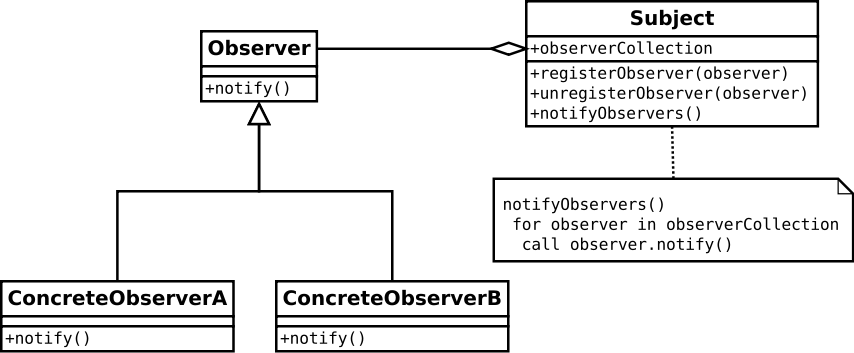
\includegraphics[width=0.9\textwidth]{images/rx.png}
                \caption{Pozorovateľ - Vydavateľ - bdiagram tried }
                \label{obr2.1}
            \end{center}
        \end{minipage}
    \end{center}
\end{figure}

Vždy ak vydavateľ zmení hodnotu, všetci pozorovatelia budú upozornení, čo je užitočné hlavne pri zobrazovaní informácií pre používateľa, každá zmena v premennej môže byť automaticky zobrazená používateľovi. Pri Http požiadavke môžeme na jednom vlákne sledovať stav požiadavky, pokiaľ požiadavka skončí, či už chybou alebo úspešne, sme schopní zobraziť informáciu používateľovi okamžite na UI vlákne.

\section{Cloudové služby}

Väčšina aplikácií komunikuje so vzdialeným serverom, ktorý odpovedá na požiadavky klienta. Nastavovanie serverovej časti aplikácie, inštalácia potrebného softvéru  a následná údržba stojí čas , ktorý je pri tvore softvéru veľmi vzácny, preto sa na trhu začali objavovať PaaS služby ktoré, vývojárovi ušetria čas.

\subsection{Heroku}
Heroku je jedna z prvých cloudových platforiem, ktorá je vyvíjaná od roku 2007. Vtedy podporovala nasadenie aplikácií len v jazyku Ruby, dnes podporuje  Javu, Node.js, Scala, Clojure, Python, PHP, a Go. Heroku poskytuje jednoduché nasadenie aplikácie priamo z verzionovacieho systému Git, ktorý poskytuje prehľad všetkých zmien v kóde. Heroku poskytuje vlastný Git repozitár, alebo napojenie na GitHub, pričom pri aktualizácii hlavnej vetvy repozitáru sa aplikácia sama skompiluje a nainštaluje. \cite{heroku}

\subsection{OpenShift}
OpenShift je PaaS produkt za ktorým stojí spoločnosť RedHat, ktorá poskystuje hosting s vývojársky prívetivými službami ako MongoDB, Node.js prístup cez webové rozhranie alebo príkazový riadok. Obsahuje všetky závislosti, potrebné na vývoj  Java Enterprise aplikácií, integráciu s IDE a automatizačnými systémami ako Maven alebo Jenkins. OpenShift dbá na zabezpečenie, preto je možné komunikovať len pomocou SSH kľúča. Rovnako ako na Heroku, aplikácia sa builduje z Git repozitáru. 

\chapter{Analýza}

\section{Klient-server} 
Architektúra klient server rozdeľuje aplikáciu na dve časti. Serverová aplikácia, ktorá je spustená na výkonnom zariadení spracováva dáta, poskytuje veľkú pamäť, alebo databázu a klientskú časť, ktorá poskytuje používateľské prostredie na odosielanie požiadaviek a zobrazenie odpovede servera\cite{clientserver}. Android aplikácie najčastejšie používajú REST architektúru, ktorá využíva URL adresu a HTTP požiadavky na interakciu so serverom. 

\begin{table}[H]
\centering
\caption{REST komunikácia}
\label{REST komun}
\begin{tabular}{|l|l|l|}
\hline
\textit{URL/Http Metóda}             & \multicolumn{1}{c|}{\textit{\textbf{GET}}} & \multicolumn{1}{c|}{\textit{\textbf{PUT}}} \\ \hline
\textit{\textbf{uniza.sk/student}}   & Vráti kolekciu študentov                   & Nahradí kolekciu novou                     \\ \hline
\textit{\textbf{uniza.sk/student/1}} & Zobrazí informácie o študentovi s id 1     & Nahradí staré údaje novými                 \\ \hline
\textit{URL/Http Metóda}             & \multicolumn{1}{c|}{\textbf{POST}}         & \multicolumn{1}{c|}{\textbf{DELETE}}       \\ \hline
\textit{\textbf{uniza.sk/student/1}} & Vytvorí novú položku a vráti jej URI       & Vymaže kolekciu                            \\ \hline
\textit{\textbf{uniza.sk/student/1}} & Vo všeobecnosti sa nepoužíva.              & Vymaže študenta z kolekcie                 \\ \hline
\end{tabular}
\end{table}

Klient posiela požiadavky na server buď pomocou URL adresy alebo s dodatočnými dátami uložené v tele požiadavky vo formáte Json, alebo XML.

\section{Základné komponenty aplikácie}
Všetky prvky operačného systému sú prístupne pre programátora pomocou API, ktoré sú naprogramované v jazyku Java. Všetky prvky tvoria stavebné bloky, ktoré potrebujeme na vývoj aplikácie. Sú to znova použiteľné a modulárne komponenty.
\subsection{Aktivita}
 
Aktivita reprezentuje jednu obrazovku, ktorá obsahuje všetky komponenty nutné pre interakciu s aplikáciou. Aktivity sú v systéme  spravované ako zásobník aktivít, nová aktivita je vždy pridaná na vrchol zásobníka, pričom predošlé aktivity ostávajú v zásobníku a nebudú zobrazené kým neodídeme z vrchnej aktivity.
Aktivita má štyri stavy. Pokiaľ je aktivita zobrazená na obrazovke je aktívna, alebo bežiaca. Ak aktivitu prekryje iné okno, ale je stále viditeľná tak je pozastavená, čo znamená, že celý jej stav je uložený a je stále aktívna. Ak je aktivita celá prekrytá novou, pôvodná je zastavená. Hoci si o sebe uchováva všetky informácie, nie je používateľovi viditeľná a môže byť kedykoľvek zmazaná z pamäte, ak systém potrebuje pamäť na inom mieste.
Nasledujúci diagram  (obr.\ref{obr1.2}.) zobrazuje životný cyklus aktivity.

\begin{figure}[H]
    \begin{center}
        \begin{minipage}{0.80\linewidth}
            \begin{center}
                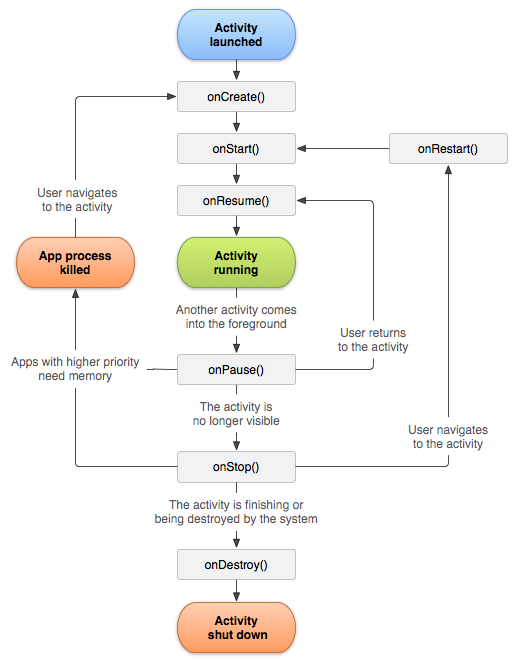
\includegraphics[width=0.85\textwidth]{images/activity_lifecycle.png}
                \caption{Životný cyklus aktivity}
                \label{obr1.2}
            \end{center}
        \end{minipage}
    \end{center}
\end{figure}

\subsection{Služba}
Service, alebo služba, je aplikačný komponent, ktorý umožňuje vykonávať dlhotrvajúce činnosti na pozadí ako je napríklad prehrávanie hudby alebo získavanie dát z GPS. Služba je spustená aplikáciou a ostáva spustená aj po jej ukončení. Má jednoduchý životný cyklus. Aplikácia ju spustí a beží až kým nie je zastavená operačným systémom, alebo spúšťajúcou aplikáciou \ref{obr1.3}.

\begin{figure}[H]
    \begin{center}
        \begin{minipage}{0.5\linewidth}
            \begin{center}
                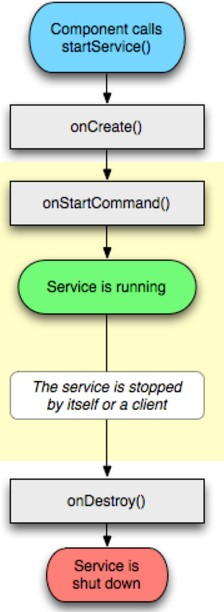
\includegraphics[width=0.5\textwidth]{images/service_life.jpg}
                \caption{Životný cyklus služby}
                \label{obr1.3}
            \end{center}
        \end{minipage}
    \end{center}
\end{figure}

\subsection{Poskytovateľ obsahu}
Poskytovateľ obsahuje spravuje dáta, ktoré môžu byť zdieľanie napriek aplikáciami pomocou  SQLite databázy. Ak má aplikácia práva, môže meniť obsah dát, ktoré sú dostupné, následne iná aplikácia dostane po vyžiadaní dát, nové a upravené hodnoty. Príklad využitia takejto služby je telefónny zoznam, kedy môže aplikácia tretej strany pristupovať k číslam, využívať ich, prípadne meniť.

 
\section{Aktuálne riešenia}
Cieľom tejto analýzy je porovnať dostupnosť, jednoduchosť a cenu súčasných najpoužívanejších riešení, ktoré sú dostupné na trhu.

  \vspace{10pt}
\subsection{JIRA Software}


\textit{JIRA Software} od spoločnosti Atlassian je software na správu projektov pre agilné tímy. Pomocou takzvaných Kanban boardov, ktoré umožňujú celému tímu vidieť aká práca ich v najbližšom období čaká, momentálne prebieha alebo je už dokončená. Jedná sa o tabuľku s kartičkami s obsahom práce, ktoré môžu následne členovia tímu premiestňovať do adekvátnych stĺpcov (obr.\ref{obr2.1}.)



\begin{figure}[ht]
    \begin{center}
        \begin{minipage}{0.99\linewidth}
            \begin{center}
                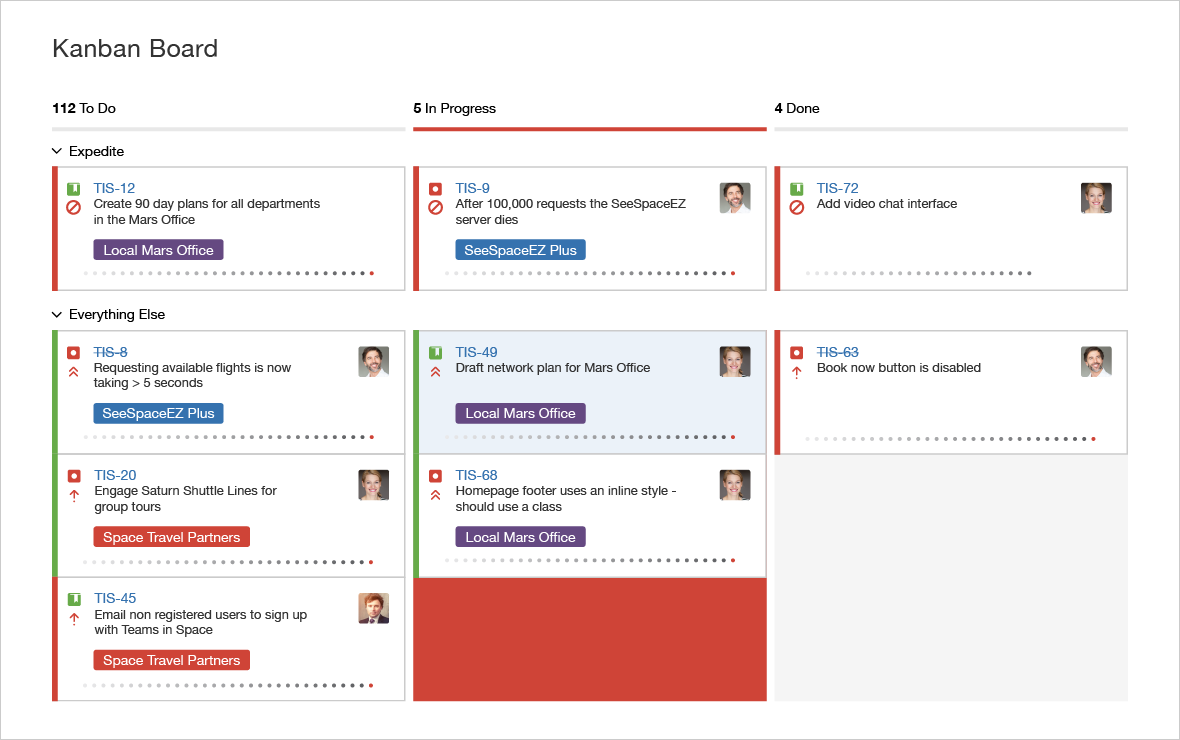
\includegraphics[width=0.99\textwidth]{images/kanbanboard.png}
                \caption{Kanban board}
                \label{obr2.1}
            \end{center}
        \end{minipage}
    \end{center}
\end{figure}

\vspace{10pt}

Každá kartička v tabuľke reprezentuje úlohu, ktorá má vždy zadávateľa a osobu, ktorá bude danú úlohu vykonávať a následne aktualizovať jej stav. Pri vytvorení a priradení úlohy príde riešiteľovi emailové oznámenie o priradení. Jedná sa o relatívne zdĺhavý proces, ktorý zamestnanci neradi vykonávajú. JIRA software je o mnoho obsiahlejší, tým pádom komplikovanejší, a napriek user-friendly prostrediu vyžaduje zaškolenie nového zamestnanca a firmy potrebujú vlastného JIRA správcu. Jedná sa ale o najobľúbenejšie riešenie pre projektový manažment ktorý umožňuje firmám lepšiu organizáciu pri riadení práce, ktorého výsledkom je kvalitný finálny produkt dodaný načas. Taktiež je rožsíriteľný o dalšie produkty spoločnosti ako sú Confluence, Bitbucket, Trello. Chýba im ale dedikovaná, jednoducha a funkčná aplikácia pre mobilné telefóny

Atlassian ponúka tri verzie ich softvéru. Verzia, ktorá sa nainštaluje na vlastný server, verzia v data centre a cloudová inštancia ich produktu. Základná verzia JIRA Core pre 25 ľudí stojí  \$1800 za serverovú aplikáciu a \$180 mesačne za cloudovú inštanciu .

\vspace{10pt}

\subsection{Slack}

\textit{Slack} je nástroj na tímovú kolaboráciu, ktorý vznikol ako interný nástroj, a v súčasnej dobe sa jedná o cloudovú službu. Jedná sa v podstate o interný chat, ktorý je rozdelený do rôznych kanálov. Kanál  (obr.\ref{obr2.2}) reprezentuje tému, projekt, lokácie alebo skupinu ľudí.


Ľudia môžu pomocou Slack-u posielať správy aj konkrétnej osobe, uskutočňovať hovory, zdieľať súbory. Externé firmy, ktoré taktiež využívajú Slack, môžu využívať spoločný kanál. Najväčšou výhodou Slack-u je, že odpadáva nutnosť odosielať hromadné maily, v ktorých sa po čase stráca prehľad, sprehľadňuje email a prenecháva mu jeho dôležitú funkciu a to  komunikáciu s  dôležitými klientmi pre formálnejší spôsob posielania správ. 
Na rozdiel od JIRA Software je Slack dostupný len z cloudu, na ktorý sa možno pripojiť cez webový prehliadač alebo aplikáciou pre všetky desktopové a mobilné platformy, pričom sa jedná o stabilné a prepracované produkty. Ponúka verziu zadarmo, ktorá ale na rozdiel od platených,  neposkytuje šifrovanie, externý prístup pre klientov alebo video konferencie.


\begin{figure}[H]
    \begin{center}
        \begin{minipage}{0.95\linewidth}
            \begin{center}
                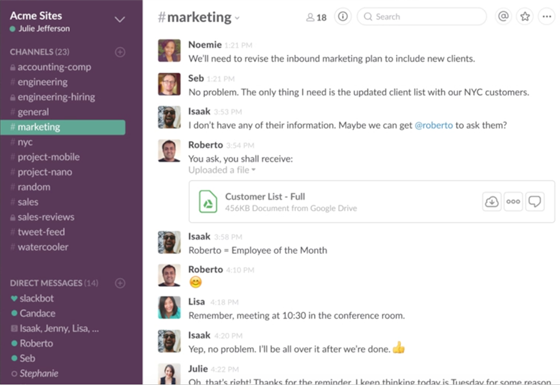
\includegraphics[width=0.99\textwidth]{images/slack.png}
                \caption{Slack, hlavné okno}
                \label{obr2.2}
            \end{center}
        \end{minipage}
    \end{center}
\end{figure}
 
\vspace{10pt}
Jedná sa o veľmi obľúbený nástroj, ktorý plní viac úlohu rýchleho chatu medzi kolegami v práci, ktorí niečo rýchlo potrebujú, ale nie sú dostatočne urgentné na telefonický rozhovor alebo posielanie mailu. 
 


\vspace{10pt}

Cieľom a úlohou tejto práce bolo navrhnúť a vytvoriť aplikáciu, ktorá by zahŕňala výhody predchádzajúcich riešení a v spojení so zadaním by bola vo finále ideálnym riešením pre malý a stredný podnik.
  
  
\section{Zber požiadaviek}

Aplikácia má poskytnúť jednoduché a intuitívne používateľské prostredie, ktoré dovolí používateľovi vidieť na akých projektoch pracuje, správy ktoré si riešitelia poslali, zapisovanie služobných ciest a jednoduchú komunikáciu medzi používateľmi. 

\begin{figure}[H]
    \begin{center}
        \begin{minipage}{0.9\linewidth}
            \begin{center}
                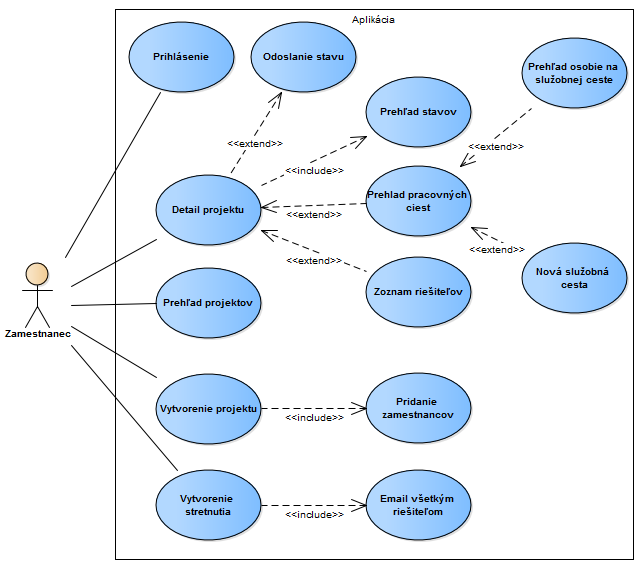
\includegraphics[width=0.9\textwidth]{images/usecase.png}
                \caption{Prípady použitia }
                \label{obr2.1}
            \end{center}
        \end{minipage}
    \end{center}
\end{figure}

Projekt by mal obsahovať všetkých ľudí ktorí na ňom pracujú, ich telefónne čísla, email a pracovnú pozíciu. Organizácia pracovného stretnutia je oznámená všetkým riešiteľom s dátumom a miestom konania na ich emailové adresy. 



